\documentclass[a4paper,10pt]{article}
\input{/home/frr/Dropbox/Modelos/Modelo_prova_latex/estilo_prova.tex}

\begin{document}


\professor{Fábio Rodrigues de la Rocha}
\turma{08655}
\codigodisciplina{ARA7560}
\disciplina{Sistemas Digitais Embarcados}
\data{11/05/2015}
\hlimite{20:20}
\tarefa{1}




\section{Introdução}

Neste texto apresenta-se o módulo Bluetooth de baixo custo JY-MCU que possui uma interface serial 
para fácil comunicação com um microcontrolador. Este módulo é vendido em dois modelos HC-06 e  HC-05. O 
HC-06 que vem de fábrica programado para ser utilizado apenas como um módulo escravo. (Em geral os dispositivos Bluetooth mouse, teclado, caixa de som são 
módulos 
escravos).  Um tablet, celular, notebook, ou um PC desktop quando possuem unidade Bluetooth 
operam como mestre. De acordo com o protocolo, os mestres que conectam nos escravos para deles capturar ou enviar os dados (teclas, movimento do mouse, audio 
para caixas de som, etc.). Para que um microcontrolador seja o mestre de um sistema Bluetooth ele precisa de um módulo HC-05 ou compatível.  

\begin{figure}[htb]
 \centering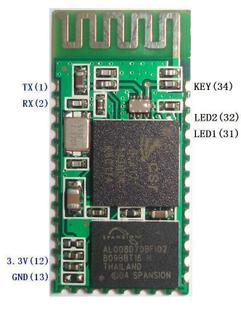
\includegraphics[width=0.4\textwidth]{placa}
\end{figure}

\subsection{Módulo escravo}

Um módulo HC-06 ou outro compatível funciona pode ser interconectado a um microcontrolador usando os pinos TX e RX do microcontrolador. O módulo atua como um dispositivo que recebe dados e transmite-os por bluetooth e que recebe dados enviados por bluetooth e os transmite para o microcontrolador. Ao iniciar um módulo escravo a sua taxa de transmissão será 9600 bits/s.



Abaixo apresenta-se um fragmento de código de um módulo escravo:

\begin{lstlisting}[numbers=none,basicstyle=\footnotesize\ttfamily]
#include <stdio.h>
#include "serial.h"

#define PINO_TX    1
#define PINO_RX    2


int main()
{
   serial_configura (PINO_TX, PINO_RX); // vai usar porta serial
   while (1)
   {
      printf("Oi mundo\r");
   }

   return 0;
}
\end{lstlisting}

\end{document}
